\documentclass[border=10pt]{standalone}
\usepackage[T1]{fontenc}
\usepackage{tikz}
\usepackage{graphicx}
\usepackage{amsmath}

\definecolor{garnet}{HTML}{73000A}
\definecolor{atlantic}{HTML}{466A9F}
\definecolor{congaree}{HTML}{1F414D}
\definecolor{warmgrey}{HTML}{676156}
\definecolor{horseshoe}{HTML}{65780B}
\definecolor{rose}{HTML}{CC2E40}
\definecolor{bk70}{HTML}{5C5C5C}
\definecolor{bk30}{HTML}{C7C7C7}
\definecolor{bk10}{HTML}{ECECEC}

\begin{document}
\begin{tikzpicture}[
    imgframe/.style={draw=bk70, thick, inner sep=0pt},
    lbl/.style={font=\sffamily\small\bfseries, text=#1},
    sublbl/.style={font=\sffamily\tiny, text=warmgrey},
    arr/.style={->, very thick, color=#1},
    eqbox/.style={draw=garnet, thick, fill=garnet!5, inner sep=6pt,
        font=\sffamily\small, text=bk70, align=center},
]

% ════════════════════════════════════════════
% Title
% ════════════════════════════════════════════

% Ultra-wide
\node[imgframe] (uw_orig) at (1.5, 6.5)
    {
\includegraphics[width=3cm]{cstm_demo/ultrawide_14mm_original.jpg}};
\node[lbl=atlantic, anchor=south] at (uw_orig.north) {Ultra-wide};
\node[sublbl, anchor=north] at (uw_orig.south) {$f = 14\text{mm}$};

% Wide
\node[imgframe] (wd_orig) at (7.5, 6.5)
    {
\includegraphics[width=3cm]{cstm_demo/wide_24mm_original.jpg}};
\node[lbl=horseshoe, anchor=south] at (wd_orig.north) {Wide (canonical)};
\node[sublbl, anchor=north] at (wd_orig.south) {$f = f^c = 24\text{mm}$};

% Tele
\node[imgframe] (tl_orig) at (13.5, 6.5)
    {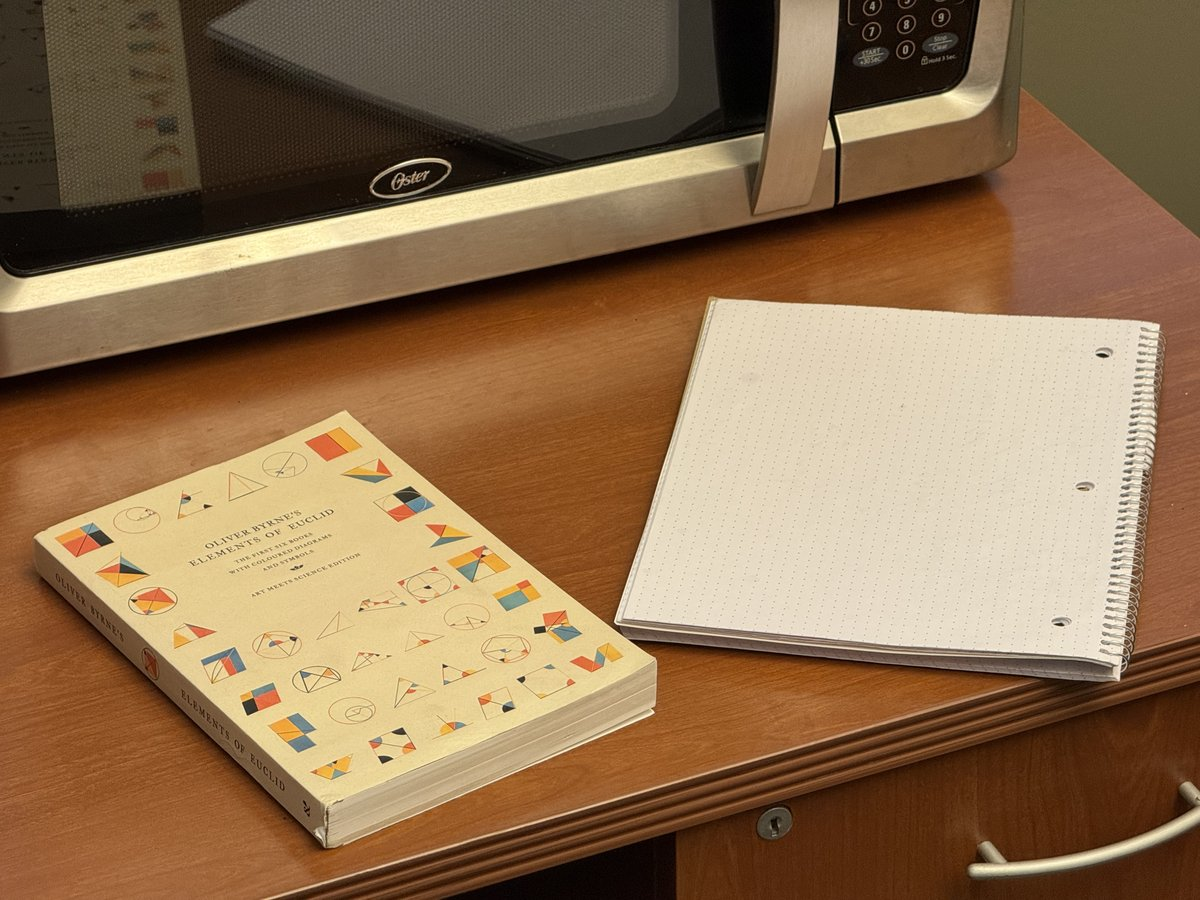
\includegraphics[width=3cm]{cstm_demo/tele_120mm_original.jpg}};
\node[lbl=rose, anchor=south] at (tl_orig.north) {Telephoto};
\node[sublbl, anchor=north] at (tl_orig.south) {$f = 120\text{mm}$};

% ════════════════════════════════════════════
% CSTM equation box (centered between rows)
% ════════════════════════════════════════════
\node[eqbox] (cstmbox) at (7.5, 3.5) {CSTM-image: $I_c = \text{resize}(I,\; \omega)$ \qquad where $\omega = f^c / f$};

% ════════════════════════════════════════════
% Arrows: originals → CSTM box
% ════════════════════════════════════════════
\draw[arr=atlantic] (uw_orig.south) -- (uw_orig.south |- cstmbox.north)
    node[midway, left, font=\sffamily\scriptsize, text=atlantic]
    {$\omega = 1.71$};

\draw[arr=horseshoe] (wd_orig.south) -- (wd_orig.south |- cstmbox.north)
    node[midway, left, font=\sffamily\scriptsize, text=horseshoe]
    {$\omega = 1.0$};

\draw[arr=rose] (tl_orig.south) -- (tl_orig.south |- cstmbox.north)
    node[midway, left, font=\sffamily\scriptsize, text=rose]
    {$\omega = 0.2$};

% ════════════════════════════════════════════
% ROW 2: CSTM-transformed images
% ════════════════════════════════════════════

% Ultra-wide (enlarged 1.71x relative to 3cm base = 5.13cm)
\node[imgframe] (uw_cstm) at (1.5, 0.8)
    {
\includegraphics[width=5.13cm]{cstm_demo/ultrawide_14mm_cstm.jpg}};
\node[sublbl, anchor=north] at (uw_cstm.south)
    {Enlarged $1.71\times$};

% Wide (unchanged, 3cm base)
\node[imgframe] (wd_cstm) at (7.5, 0.8)
    {
\includegraphics[width=3cm]{cstm_demo/wide_24mm_cstm.jpg}};
\node[sublbl, anchor=north] at (wd_cstm.south)
    {Unchanged};

% Tele (shrunk 0.2x relative to 3cm base = 0.6cm)
\node[imgframe] (tl_cstm) at (13.5, 0.8)
    {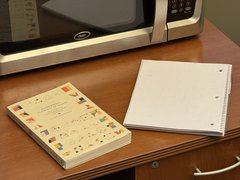
\includegraphics[width=0.6cm]{cstm_demo/tele_120mm_cstm.jpg}};
\node[sublbl, anchor=north] at (tl_cstm.south)
    {Shrunk $0.2\times$};

% Arrows: CSTM box → results
\draw[arr=atlantic] (uw_cstm.north |- cstmbox.south) -- (uw_cstm.north);
\draw[arr=horseshoe] (wd_cstm.north |- cstmbox.south) -- (wd_cstm.north);
\draw[arr=rose] (tl_cstm.north |- cstmbox.south) -- (tl_cstm.north);

% ════════════════════════════════════════════
% Bottom: result label
% ════════════════════════════════════════════

\end{tikzpicture}
\end{document}
